\documentclass[11pt, a4paper]{report}
\usepackage{polski}
\usepackage[cp1250]{inputenc}
\usepackage{color}
\usepackage[table]{xcolor}
\usepackage{listings}
\usepackage{caption}
\usepackage{enumitem}
\usepackage{graphics}
\usepackage{epsfig}
\usepackage{rotating}
\usepackage{fancyhdr}
\usepackage{subfig}
\usepackage{url}
\usepackage{float}

\restylefloat{figure}

\renewcommand{\figurename}{Rys.}
\renewcommand{\tablename}{Tab.}
\renewcommand{\lstlistlistingname}{Spis listing�w}


%% Define a new 'leo' style for the package that will use a smaller font.
\makeatletter
\def\url@leostyle{%
  \@ifundefined{selectfont}{\def\UrlFont{\sf}}{\def\UrlFont{\small\ttfamily}}}
\makeatother
%% Now actually use the newly defined style.
\urlstyle{leo}

\pagestyle{fancy}


\pagestyle{fancy}
\rhead{}
\lhead{\nouppercase{\leftmark}}



\lstdefinelanguage{apache}{
morekeywords={ServerAdmin, ServerName, ServerAlias, DocumentRoot, Options, AllowOverride, Order, ErrorLog, LogLevel, CustomLog, allow},
sensitive=false,
morestring=[b]"
}

\definecolor{bbb}{gray}{0.90}

\newcommand{\lstMikro}[1]
{\lstinline[breakatwhitespace=true, postbreak=\kern-3ex, basicstyle=\small\ttfamily,breaklines=true,language=bash,literate={\`}{}{0\discretionary{-}{}{}}]$#1$}

\lstset{
         basicstyle=\scriptsize\ttfamily, % Standardschrift
			numbers=left,
         numberstyle=\tiny,          % Stil der Zeilennummern
         %stepnumber=2,               % Abstand zwischen den Zeilennummern
         numbersep=5pt,              % Abstand der Nummern zum Text
         tabsize=2,                  % Groesse von Tabs
         extendedchars=true,         %
         breaklines=true,            % Zeilen werden Umgebrochen
         keywordstyle=\color{blue},
         stringstyle=\color{red}\ttfamily, % Farbe der String
         xleftmargin=17pt,
         framexleftmargin=17pt,
         framexrightmargin=6pt,
			framextopmargin=0pt,
         backgroundcolor=\color{bbb},
         showstringspaces=false     % Leerzeichen in Strings anzeigen ?        
 }



\DeclareCaptionFont{white}{\color{white}}
\DeclareCaptionFormat{listing}{\colorbox{gray}{\parbox{\textwidth}{#1#2#3}}}
\captionsetup[lstlisting]{format=listing,labelfont=white,textfont=white}

\makeatletter
\newcommand{\linia}{\rule{\linewidth}{0.4mm}}

% new itemize environment with itemsep parameter
\newenvironment{packed_item}[1][0]
  { \begin{itemize}
    % set spacing between items
    \addtolength{\itemsep}{#1\baselineskip}
    % set spacing between lines
    \addtolength{\baselineskip}{#1\baselineskip} }
  { \end{itemize} }


\renewcommand{\maketitle}{\begin{titlepage}

    \vspace*{1cm}

    \begin{center}\small
    Politechnika ��dzka\\
    Wydzia� Fizyki Technicznej i Matematyki Stosowanej\\
    Informatyka\\
    Systemy Informatyczne i Bazy Danych
    \end{center}

    \vspace{3cm}

    \noindent\linia

    \begin{center}

      \LARGE \textsc{\@title}

         \end{center}

     \linia

    \vspace{0.5cm}

    \begin{flushright}

    \textit{\small Autor:}\\

    \normalsize \textsc{\@author} \par

    \vspace{1cm}

     \textit{\small Opiekun:}\\

         dr in�. Anety Poniszewska - Mara�da
		
     \end{flushright}

    \vspace*{\stretch{6}}

    \begin{center}

    \@date

    \end{center}

  \end{titlepage}%

}

\makeatother

\title{Optymalizacja wydajno�ci aplikacji internetowych}
\author{�ukasz Adamczewski}
\begin{document}


\includepdf[pages={1}]{tytul.pdf}

    %podzi�kowania
    \newpage
    ~   %potrzebne dla \vfill
    \vfill
    {\sffamily
    \begin{flushright}
        \begin{tabular}{l}
        Chcia�bym w~tym miejscu podzi�kowa�:\\
        \\
        Narzeczonej Oliwii\\
        za wsparcie i wyrozumia�o�� podczas pisania pracy\\
        \\
        Rodzicom\\
        za pomoc w rozwijaniu pasji,\\dbaj�c o kondycje zdrowia psychicznego\\
			\\
        Pani promotor dr in�. Anecie Poniszewskiej - Mara�dzie\\
        za wnikliw� analiz� i pomoc podczas pisania pracy.\\
        \end{tabular}
    \end{flushright}
    }
    \vskip0.5in
    \thispagestyle{empty}
    \newpage
    %koniec podzi�kowa�

\tableofcontents


\addcontentsline{toc}{chapter}{Wst�p}
\chapter*{Wst�p}

Obecnie Internet przesta� ju� by� tylko wojskowym eksperymentem lub zaledwie miejscem na publikacje w�asnej strony domowej. Wyewoluowa� do medium globalnej komunikacji z gigantyczn� ilo�ci� klient�w docelowych. Wi�kszo�� firm, instytucji lub organizacji rz�dowych czuje si� w obowi�zku posiadania i utrzymywania strony internetowej, zazwyczaj spe�niaj�cej okre�lone cele biznesowe. Pokazuje to jak bardzo powszechnym narz�dziem codziennego u�ytku jest dzisiaj globalna paj�czyna.\\


\section*{Problematyka pracy}

Wraz ze wzrostem popularno�ci Internetu jako medium informacyjnego, istotnym problemem sta�o si� obs�u�enie nap�ywaj�cego ruchu sieciowego ze strony u�ytkownik�w. Poj�cie "czas to pieni�dz" ma tutaj kluczowe znaczenie, poniewa� umiej�tno�� przetworzenia jak najwi�kszej ilo�ci u�ytkownik�w w jak najkr�tszym czasie b�dzie przek�ada�a si� na realne zyski.

Innym wa�nym problemem dotycz�cym stron jest zapewnienie wysokiej dost�pno�ci us�ugi, czyli wyeliminowanie do minimum wszelkiego rodzaju przerw wynikaj�cych z b��d�w aplikacji. Temat ten zwi�zany jest jednak g��wnie z odpowiedni� konfiguracj� sprz�tow�, czyli wykorzystaniem r�wnolegle dzia�aj�cych instancji sprz�towych, kt�re b�d� wykorzystywane w celu zr�wnowa�enia ruchu lub awaryjnie w wypadku uszkodzenia no�nika danych na jednym z urz�dze�.\\

Nale�y zaznaczy� na wst�pie, �e statystycznie tylko\textbf{ 20\%} czasu przetwarzania strony przez przegl�dark�, jest po�wi�cane na oczekiwanie na odpowied� serwera. Implikuje to olbrzymie znaczenie optymalizacji kodu po stronie klienta w celu znacznego przyspieszenia czasu odpowiedzi strony. 
Nie bez znaczenia s� te� czynniki, takie jak lokalizacja geograficzna oraz konfiguracja serwera.\\

Ze wzgl�du na niekwestionowan� popularno�� j�zyka PHP (wed�ug bada� z drugiej po�owy sierpnia 2012 roku udzia� wynosi a� \textbf{77.8\%}) \cite{phpUsage} oraz jego olbrzymi� prostot� - w stosunkowo kr�tkim czasie od powstania j�zyka, zacz�y pojawia� si� proste strony, nast�pnie aplikacje internetowe, a ko�cz�c na portalach i us�ugach sieciowych. J�zyk PHP sta� si� narz�dziem na tyle uniwersalnym, �e zagadnienia modelowane przy jego u�yciu, mo�na z powodzeniem przenie�� na inne platformy, takie jak \textit{Java Enterprise} lub \textit{.NET}. W sieci istnieje ponadto wiele gotowych implementacji system�w e-commerce: sklep�w (na przyk�ad Magento czy osCommerce), system�w CRM (SugarCRM) lub na przyk�ad platforma edukacyjna Moodle, b�d�ca cz�ci� infrastruktury edukacyjnej Politechniki ��dzkiej. Wymienione przyk�ady zosta�y w ca�o�ci zaimplementowane w j�zyku PHP, a o ich popularno�ci �wiadcz� miliony �ci�gni�� i wdro�e�.\\

Jedn� z wad gotowych rozwi�za� jest fakt, �e nie zawsze s� one dostosowane do wszystkich stawianych przed projektem wymaga�. Powoduje to, �e, projekt docelowy w rezultacie otrzyma wi�cej funkcjonalno�ci ni� jest to wymagane. Z drugiej jednak strony mo�liwe jest, �e gotowe rozwi�zanie b�dzie wymaga�o szeregu usprawnie� lub dodania nowych funkcjonalno�ci. W wi�kszo�ci wypadk�w, rozwi�zania gotowe nie s� jednak od pocz�tku dostosowane do bardziej zaawansowanych zastosowa� lub wymaga� wydajno�ciowych. Dlatego wa�ne jest, by wykorzystuj�c istniej�ce narz�dzia wyskalowa� aplikacje do konkretnych potrzeb lub przewidzie� przysz�e obci��enie.\\

Ponadto, poza j�zykiem PHP, dzi�ki stworzeniu platformy \textit{Google Application Engine}, j�zyk Python zyska� du�� popularno�� w�r�d dost�pnych rozwi�za�. Jest on uwa�any za j�zyk, w kt�rym mo�na pisa� �atwy w utrzymaniu kod w bardzo kr�tkim czasie, wszystko dzi�ki wbudowanym mechanizmom i wieloletniemu do�wiadczeniu tw�rc�w \cite{book:python}.

Analiza wydajno�ciowa przeprowadzana w wypadku prostych aplikacji, kt�re nie b�d� w przysz�o�ci podlega�y intensywnemu obci��eniu nie ma w zasadzie sensu. Publikacja zyskuje na warto�ci w wypadku, kiedy projekt jest bardziej rozbudowany, a my potrzebujemy szybkiego i rzetelnego sposobu na wykrycie potencjalnych obszar�w do optymalizacji.
Problem wydajno�ci aplikacji bardzo cz�sto ujawnia si� w trudnych do przewidzenia momentach, dlatego kluczow� umiej�tno�ci� jest nauka analizy log�w systemowych, udost�pnianych przez dostawc�w.


\section*{Cel pracy}

W internecie istnieje stosunkowo du�o publikacji zwi�zanych z tematyk� optymalizacji aplikacji webowych, jednak�e w wi�kszo�ci wypadk�w omawiany jest tylko nik�y procent wszystkich zagadnie�. 
Zazwyczaj pomijane s� aspekty zwi�zane z kodem po stronie klienta, a tak�e studium narz�dzi i metod badawczych. Najpopularniejsze s� publikacje dotycz�ce optymalizacji samego kodu lub zapyta� bazodanowych, w zale�no�ci od u�ytego j�zyka aplikacji lub bazy danych.\\

Praca ma na celu przedstawienie mo�liwie najszerszego wachlarza technik optymalizacji. W ramach pracy planowane jest po��czenie kilku technologii i wymiana danych mi�dzy nimi z wykorzystaniem �atwiejszych do przetworzenia obiekt�w JSON (ang. \textit{JavaScript Object Notation}). Jest to lekki format wymiany danych, natywnie interpretowany przez j�zyk \textit{JavaScript}.

Jednym z cel�w jest r�wnie� przedstawienie stosunkowo nowych us�ug sprz�towo - programistycznych znanych jako \textit{PAAS} (ang. \textit{Platform as a Service}). Takie rozwi�zania daj� mo�liwo�� elastycznego dostosowywania zaplecza sprz�towego do bie��cych potrzeb.

Praca ma r�wnie� na celu prezentacj� narz�dzi, umo�liwiaj�cych znalezienie w�skich garde� aplikacji. Tylko sukcesywne ��czenie r�nych narz�dzi oraz ci�g�e monitorowanie dzia�ania, zapewni oprogramowaniu stabilno�� oraz wysok� dost�pno��.



\section*{Zakres pracy}

Niniejsza praca dyplomowa dotyczy zagadnie� in�ynierii oprogramowania oraz technologii baz danych wykorzystanych w dziedzinie \textit{e-commerce}. G��wny cel bada� stanowi przedstawienie realnych korzy�ci biznesowych wynikaj�cych z zastosowania szerokiego spektrum usprawnie� aplikacji internetowych. 

Tre�� pracy dyplomowej stanowi "wypadkow�" informacji zawartych w dokumentacjach dotycz�cych u�ytych technologii, jak r�wnie� wiedzy autora zdobytej podczas implementacji wielu zr�nicowanych aplikacji internetowych. Bardzo istotne dla publikacji by�y r�wnie� informacje pochodz�ce ze sprawdzonych �r�de�, takich jak na przyk�ad oficjalny blog programistyczny Yahoo. Serwis Yahoo ze wzgl�du na olbrzymie do�wiadczenie w kwestii skalowania aplikacji internetowych postanowi� podzieli� si� t� wiedz� na �amach swoich stron internetowych oraz kilku specjalistycznych ksi��ek.\\

Wiele stron takich jak \texttt{Twitter} czy \texttt{Facebook} na swoich blogach dzieli si� do�wiadczeniami zwi�zanymi z implementacj� i problemami zwi�zanymi z wydajno�ci�. Jest to kolejne cenne �r�d�o informacji o sposobach poprawy dzia�ania aplikacji.

W tre�ci pracy przedstawiona jest analiza technik optymalizacji aplikacji internetowych z uwzgl�dnieniem wykonywanych po stronie serwera (\textit{server side}) oraz szeregu usprawnie� po stronie przegl�darki \textit{client side}. 
R�wnie istotny jest wyb�r metod, daj�cych najlepsze rezultaty w �wietle obecnych technologii. Dodatkowo, wa�ne jest wyr�nienie wszystkich po�rednich czynnik�w, kt�re mog� w jakimkolwiek stopniu wp�yn�� na dzia�anie aplikacji.\\

Do implementacji systemu wykorzystano technologie skryptowe PHP oraz Python. 
Pierwsza z nich pozwoli na szybkie przedstawienie obrazu typowej aplikacji e-commerce (olbrzymi odsetek takich aplikacji w Internecie jest napisanych w�a�nie w tym j�zyku). Python z kolei pozwoli wykorzysta� zalety platformy Google Application Engine (GAE), kt�ra zapewnia skalowaln� architektur� do p�niejszych test�w.

Obserwacja zostanie przeprowadzona na przyk�adzie prostej aplikacji z dziedziny \textit{e-commerce} - ksi�garni elektronicznej. Wyb�r takiej tematyki jest celowy, poniewa� najcz�ciej w�a�nie w takich aplikacjach wyst�puj� problemy natury optymalizacyjnej. Spowodowane jest to najcz�ciej konieczno�ci� obs�u�enia wielu klient�w, transakcji bazodanowych lub przede wszystkim generowanie rozbudowanego wizualnie interfejsu u�ytkownika. Podczas generowania obraz�w, wykonywania kodu serwera, czy interpretowania rozbudowanych struktur dokumentu \textit{HTML}, czas oczekiwania na wynik mo�e si� zauwa�alnie wyd�u�y�.\\

Zaprojektowana w ramach pracy aplikacja stanowi studium przypadku analizy wydajno�ciowej aplikacji dzia�aj�cej w �ci�le okre�lonej architekturze. W ramach analizy om�wione zostan� nast�puj�ce zagadnienia:
\begin{packed_item}[-0,2]
	\item metody badawcze wydajno�ci aplikacji
    \item dob�r odpowiedniej technologii,
	 \item wyb�r w�a�ciwej architektury sprz�towej,
    \item projekt i optymalizacja bazy danych,
	 \item optymalizacja kodu klienta,
	 \item optymalizacja aplikacji i testy wydajno�ci
\end{packed_item}


\section*{Uk�ad pracy}
\label{sec:uklad-pracy}

Praca zosta�a podzielona na nast�puj�ce rozdzia�y:\\
\begin{itemize}
    \item \textbf{Rozdzia� pierwszy} opisuje narz�dzia badaj�ce wydajno�� aplikacji, a tak�e wyja�nia teori� dzia�ania aplikacji opartych o protok� HTTP
	\item \textbf{W drugim rozdziale} przedstawiono wymagania stawiane przed stworzon� aplikacj� oraz jej budow�.
	\item \textbf{Trzeci rozdzia�} dotyczy optymalizacji zwi�zanej z wyborem odpowiedniej architektury aplikacji.
	\item \textbf{Rozdzia� czwarty} dotyczy optymalizacji zwi�zanej z implementacj� aplikacji.
	\item \textbf{Rozdzia� pi�ty} dotyczy optymalizacji kodu klienckiego.
	\item \textbf{Rozdzia� sz�sty} to podsumowanie i wnioski ko�cowe.
	
\end{itemize}

\chapter{Analiza jako�ciowa i wydajno�ciowa aplikacji}

Projektuj�c aplikacje, ju� fazy projektowej, nale�y my�le� o zapewnieniu wysokiej wydajno�ci, a tak�e o potencjalnych problemach, kt�re mog� si� pojawi� po wdro�eniu oprogramowania. W celu zapewnienia tworzonej aplikacji najwy�szej skuteczno�ci pracy, nale�y wzi�� pod uwag� wiele cech, w�r�d kt�rych najwa�niejsze zdefiniowane s� poni�ej.

\begin{description}
\item[Skalowalno�� (ang. \textit{Scalability})] cecha aplikacji, okre�lana jako zdolno�� do wzrostu wydajno�ci aplikacji. Wraz ze zwi�kszeniem ilo�ci dost�pnych zasob�w sprz�towych (serwery WWW, bazy danych, wydajniejsze procesory).

\item[Niezawodno�� (ang. \textit{High availability})] stanowi projekt, jak i odpowiedni� implementacje systemu, zapewniaj�ca okre�lony poziom ci�g�o�ci wykonywania operacji w czasie. Polega to na zapewnieniu jak najwi�kszej dost�pno�ci us�ugi.

\item[Wydajno�� (ang. \textit{Performance})] przek�ada si� na mo�liwo�� faktycznego obs�u�enia du�ego ruchu sieciowego, przy jednoczesnym utrzymaniu czasu odpowiedzi aplikacji na stosownym poziomie.
\end{description}

Cz�sto skalowalno�� jest mylona z wydajno�ci�, jednak przek�adaj�c to na bardziej �yciowy przyk�ad, wydajno�� aplikacji mo�na por�wna� do szybkiego samochodu. Z drugiej strony, bez zapewnienia odpowiednich dr�g, ten szybki samoch�d lub ich grupa, nie jest w stanie rozwin�� maksymalnej pr�dko�ci. W najgorszym wypadku mo�e nawet utkwi� w korku, blokowany przez inne pojazdy. 
Skalowalno�� jest wi�c zapewnieniem \textbf{odpowiedniej infrastruktury} gwarantuj�cej w�a�ciwy rozrost systemu.\\

W celu zapewnienia mo�liwie najlepszej jako�ci tworzonej aplikacji, nale�y stale monitorowa� aktualny poziom wydajno�ci aplikacji. Nale�y jednak mie� na uwadze, �e na wydajno�� aplikacji sk�ada si� czas przetwarzania poszczeg�lnych w�z��w systemu. Nale�y wi�c testowa� ka�de z nich osobnymi metodami, om�wionymi w dalszej cz�ci pracy.

Szukaj�c przyczyn b��d�w, warto rozpocz�� analiz� od najbardziej og�lnego komponentu czyli serwera WWW odpowiedzialnego za wysy�anie odpowiedzi na ��danie u�ytkownika. Nast�pnie nale�y dokona� dekompozycji, wyr�niaj�c kolejne w�z�y systemu, takie jak dalsze instancje serwera WWW czy serwery bazodanowe.

\section{Analiza wydajno�ci serwera WWW}

Zadaniem serwera WWW jest wys�anie do inicjatora ��dania wyniku przetwarzania zasobu okre�lonego adresem URL. W najprostszym wypadku, analiza wydajno�ci serwera, polega na odpytaniu go o okre�lony zas�b i zmierzenie czasu od rozpocz�cia tej akcji, do odebrania rezultatu. Taki proces mo�ma prze�ledzi� i przeanalizowa� w wi�kszo�ci popularnych przegl�darek np. Google Chrome, kt�re jest wyposa�one w wiele przydatnych narz�dzi analitycznych (Rys. \ref{fig:rys1_chrome}).

\begin{figure}[htbp]
\caption{Analiza czasu wykonywania strony http://ftims.edu.p.lodz.pl// wykonana w przegl�darce Google Chrome}
\label{fig:rys1_chrome}
\includegraphics[scale=0.71]{rys1_chrome.pdf}
\end{figure}

Taki spos�b analizy, jest jednak przydatny jedynie w wypadku znacznych problem�w z wydajno�ci� aplikacji, poniewa� testowanie czasu odpowiedzi dla pojedynczego u�ytkownika, wykonuj�cego pojedyncze ��danie, nie jest w �adnym stopniu miarodajne.\\

W celu zapewnienia bardziej rzetelnego testu, nale�y skorzysta� z dedykowanych rozwi�za� takich jak \texttt{ab} oraz \texttt{siege}. 
S� to typowe narz�dzia przeznaczone do sprawdzania jak dobrze serwer radzi sobie z obs�ug� bardziej z�o�onego ruchu sieciowego. 
Przyk�adowo, dla wcze�niej u�ytej strony, mo�na zasymulowa� ruch r�wny wykonaniu 10 jednoczesnych ��da� przez 10 niezale�nych u�ytkownik�w. 
W tym celu nale�y wyda� komend� \lstinline{ab -n 10 -c 10 http://ftims.edu.p.lodz.pl/}. Rezultat dzia�ania komendy widoczny jest na listingu \ref{listing:ab}.

\begin{lstlisting}[caption=Analiza strony z wykorzystaniem narz�dzia \texttt{ab}, label=listing:ab]
Server Software:        Apache/2.2.14
Server Hostname:        ftims.edu.p.lodz.pl
Server Port:            80

Document Path:          /
Document Length:        48759 bytes

Concurrency Level:      10
Time taken for tests:   0.695 seconds
Complete requests:      10
Failed requests:        0
Write errors:           0
Total transferred:      492510 bytes
HTML transferred:       487590 bytes
Requests per second:    14.38 [#/sec] (mean)
Time per request:       695.270 [ms] (mean)
Time per request:       69.527 [ms] (mean, across all concurrent requests)
Transfer rate:          691.77 [Kbytes/sec] received

Connection Times (ms)
              min  mean[+/-sd] median   max
Connect:       52   63   7.4     63      74
Processing:   300  503  90.9    532     632
Waiting:      127  233  62.8    235     381
Total:        354  565  92.9    593     695

Percentage of the requests served within a certain time (ms)
  50%    593
  66%    612
  75%    625
  80%    628
  90%    695
  95%    695
  98%    695
  99%    695
 100%    695 (longest request)

\end{lstlisting}

Jak mo�na wywnioskowa� z powy�szych danych, narz�dzie wykonuje wiele przydatnych analiz, a tak�e wy�wietla informacje o badanym zasobie. 
Wida� przede wszystkim, �e czas oczekiwania na stron� przy 10 u�ytkownikach jest prawie trzykrotnie d�u�szy, ni� podczas jednego ��dania wykonanego w przegl�darce (\ref{fig:rys1_chrome}). 

Oczywi�cie na wyniki pomiar�w ma tak�e wp�yw pr�dko�� po��czenia internetowego, dlatego w celu pomini�cia dodatkowych czynnik�w, testy docelowej aplikacji b�d� wykonywane przede wszystkim na lokalnym serwerze. 
Najbardziej miarodajn� jednostk� okre�laj�c� wydajno�� aplikacji w wypadku narz�dzia \textit{ab} jest liczba zapyta� na sekund� (\textit{req/s}). 
Okre�la ona maksymaln� ilo�� ��da� w jednostce czasu, jak� aplikacja jest w stanie obs�u�y�. Oczywi�cie im wi�ksza warto��, tym lepsza og�lna wydolno�� aplikacji.\\

Na rysunku \ref{fig:rys2_http_lifecycle} przedstawiono cykl �ycia ��dania od u�ytkownika je inicjuj�cego, ko�cz�c na odebraniu odpowiedzi serwera. Jak mo�na zauwa�y� ��danie przebywa stosunkowo d�ug� drog�, nim trafi do faktycznej aplikacji. Wynikiem tego s� dodatkowe op�nienia zale�ne od stopnia skomplikowania architektury trzech pierwszych w�z��w. 
Dlatego te� nale�y mie� na uwadze, �e problemy z szybko�ci� dzia�ania aplikacji nie musz� le�e� wy��cznie po stronie aplikacji lub serwera. 
Do najbardziej popularnych nale��: niska przepustowo�� ��cza internetowego klienta, wolny serwer DNS, daleka lokalizacja geograficzna serwera WWW, �le skonfigurowany router lub bardzo obci��ona sie� lokalna.

\begin{figure}[htbp]
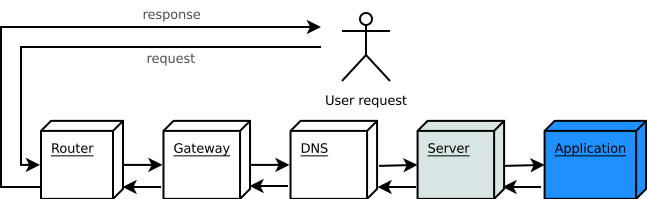
\includegraphics[scale=0.55]{fig_request.pdf}
\caption{Cykl �ycia ��dania}
\label{fig:rys2_http_lifecycle}
\end{figure}

Nawi�zuj�c do listingu \ref{listing:ab}, warto�ciami zwi�zanymi ze wspomnianymi w poprzednim akapicie w�z�ami s� \texttt{Connect} oraz \texttt{Waiting}, czyli odpowiednio czas oczekiwania na po��czenie z zasobem i czas pobierania odpowiedzi z zasobu. Istnieje 5 g��wnych czynnik�w wp�ywaj�cych na czas odpowiedzi serwera.

\begin{description}

\item[Po�o�enie geograficzne i problemy z sieci� komputerow�.]

Nie bez znaczenia dla czasu odpowiedzi, jaki u�ytkownik odczuwa jest te� lokalizacja serwer�w stron. Je�li serwery s� zlokalizowane w USA, a u�ytkownicy odwiedzaj�cy stron� s� np. z Europy, dystans jaki musi pokona� ��danie od momentu dotarcia do zasobu, oczekiwania, a� do jego pobrania jest nie wsp�miernie wi�kszy ni� w wypadku stron hostowanych dla tego samego po�o�enia geograficznego. 
Stopie� op�nienia jest zazwyczaj uzale�niony od ilo�ci router�w, serwer�w po�rednich, a nawet ocean�w, kt�re pokonuje ��danie od punktu pocz�tkowego do odbiorcy i z powrotem.

\item[Wielko�� dokumentu odpowiedzi serwera.] Zale�no�� mi�dzy wielko�ci� dokumentu, a czasem odpowiedzi serwera jest oczywista, �atwo wi�c sprawdzi�, �e im wi�kszy dokument trzeba pobra�, tym wi�cej czasu potrzeba na zako�czenie tego procesu.

\item[Wykonywanie kodu aplikacji.] Najcz�stsza przyczyna wolnego dzia�ania aplikacji wynika w�a�nie z braku optymalizacji kodu klienta. D�ugi czas wykonywania kodu aplikacji implikuje, d�ugi czas ��czny oczekiwania na odpowied� serwera. Problem ten zostanie szczeg�owiej poruszony w rozdziale \ref{cha:optymalizacja_aplikacji}.

\item[Rodzaj u�ytej przegl�darki.] Nie bez znaczenia dla og�lnego czasu �adowania strony jest r�wnie� rodzaj u�ytej przegl�darki. Cz�sto wbudowane w przegl�dark� wewn�trzne mechanizmy buforowania zasob�w pozwalaj� w znaczny spos�b zredukowa� ilo�� zapyta� wysy�anych do serwera. Dotyczy to zw�aszcza danych statycznych takich jak arkusze CSS, pliki JavaScript czy zasoby graficzne, kt�re nie zmieniaj� si� zbyt cz�sto. 

\item[Konfiguracja serwera WWW.] W zale�no�ci od u�ytej technologii, istnieje wiele r�nych serwer�w HTTP. W�r�d najcz�ciej u�ywanych, prym wiedzie serwer HTTP \textit{Apache}. 
Dla rozwi�za� napisanych w technologii Java cz�sto wykorzystywane s� serwery \textit{GlassFish}, \textit{Tomcat}, \textit{Jetty}. W wi�kszo�ci wypadk�w zaraz po instalacji, oprogramowanie serwera nie nadaje si� jeszcze do wykorzystania w produkcji. 
Nale�y wywa�y� ustawienia serwera do bie��cych potrzeb, poniewa� w wi�kszo�ci wypadk�w domy�lne ustawienia mog� znacznie obni�y� og�ln� wydajno��. 
Innym wa�nym dzia�aniem jest dostosowywanie serwera do konkretnych zastosowa� - do serwowania plik�w statycznych lepszym rozwi�zaniem jest wykorzystanie bardziej oszcz�dnego pami�ciowo i operacyjnie serwera \textit{Ngnix}, natomiast do bardziej zaawansowanych zastosowa�, w tym wykonywanie kodu aplikacji, serwera Apache lub osobnej instancji serwera \textit{Ngnix}.

\end{description}

Administratorzy serwer�w WWW maj� bezpo�redni dost�p do statystyk odwiedzalno�ci stron, przez co pozwala to zaobserwowa� pewne trendy odwiedzin u�ytkownik�w. 
Cz�sto jest tak, �e dane zasoby s� du�o intensywniej odpytywane przez u�ytkownik�w np. w czasie 10 minut stron� odwiedza 100 u�ytkownik�w. 
�atwo to sobie wyobrazi� np. w wypadku premiery jakiej� nowej gry, lub publikacji wynik�w egzaminu na uczelni. 
Taki periodyczny, lecz bardzo wzmo�ony ruch mo�e powodowa� pewne trudne do ustalenia problemy z dzia�aniem aplikacji. Dlatego te� tw�rcy narz�dzia \texttt{ab}, zaimplementowali r�wnie� mo�liwo�� test�w czasowych (ang. \textit{timed tests}). W ten spos�b mo�na zasymulowa� jak strona b�dzie si� zachowywa�a r�wnie� w takich nag�ych wypadkach.\\

Wydaj�c komend� \lstinline{ab -c 10 -t 30 http://ftims.edu.p.lodz.pl/}, mo�na sprawdzi�, jak zachowa si� aplikacja odwiedzana przez 10 u�ytkownik�w jednocze�nie w czasie 30 sekund. Ta komenda pozbawiona jest parametru \textit{-t ilo�� ��da�}, oznacza to �e symulacja zako�czy si� po 30 sekundach lub po osi�gni�ciu limitu 50 000 ��da�.

\begin{lstlisting}[caption=Test obci��enia czasowego, label=listing:ab_2]
Benchmarking ftims.edu.p.lodz.pl (be patient)
Finished 504 requests

Server Software:        Apache/2.2.14
Server Hostname:        ftims.edu.p.lodz.pl
Server Port:            80

Document Path:          /
Document Length:        48759 bytes

Concurrency Level:      10
Time taken for tests:   40.180 seconds
Complete requests:      504
Failed requests:        0
Write errors:           0
Total transferred:      24822504 bytes
HTML transferred:       24574536 bytes
Requests per second:    12.54 [#/sec] (mean)
Time per request:       797.213 [ms] (mean)
Time per request:       79.721 [ms] (mean, across all requests)
Transfer rate:          603.31 [Kbytes/sec] received

Connection Times (ms)
              min  mean[+/-sd] median   max
Connect:       48   65  14.3     61     145
Processing:   284  436 288.9    376    2957
Waiting:      119  199 281.5    151    2660
Total:        333  500 287.8    439    3007

Percentage of the requests served within a certain time (ms)
  50%    439
  66%    458
  75%    477
  80%    493
  90%    563
  95%    666
  98%   1420
  99%   2142
 100%   3007 (longest request)

\end{lstlisting}

Listing \ref{listing:ab_2} przedstawia wynik test�w czasowych. Najwa�niejsz� informacj� z punktu widzenia optymalizacji jest ilo�� ��da� na sekund�, kt�ra w tym wypadku wynosi \texttt{12.54}. Narz�dzie \texttt{ab} pozwala r�wnie� zdiagnozowa� potencjalne b��dy aplikacji pod wp�ywem zbyt du�ego ruchu. 
Pola takie jak \texttt{Failed requests} oraz \texttt{Write errors} u�atwiaj� okre�lenie prawid�owo�ci wykonywania ��da�. W powy�szym przyk�adzie, warto�ci s� akceptowalne (�redni czas ��dania to 0.5 sekundy), co najwa�niejsze nie wyst�puj� b��dy na poziomie serwera WWW i z du�ym prawdopodobie�stwem r�wnie� na poziomie aplikacji. Oczywi�cie zauwa�alny jest spadek wydajno�ci, w por�wnaniu z pierwszym testem, co prawda warto�ci �rednie s� zbli�one, jednak wida� wi�ksze rozbie�no�ci mi�dzy warto�ciami minimalnymi a maksymalnymi. Najd�u�sze zapytanie zaj�o ponad 3 sekundy. 

W dokumentacji aplikacji \texttt{ab}, mo�na znale�� informacj�, �e niekt�re serwery mog� blokowa� wysy�ane przez niego nag��wki HTTP. 
W tym celu mo�na wykorzysta� prze��cznik umo�liwiaj�cy podanie si� za inn� przegl�dark�. 
Np. chc�c zasymulowa� odwiedziny przy u�yciu przegl�darki Chrome nale�y wykona� poni�sz� komend�.
\lstinline{ab -n 100 -c 5 -H "Mozilla/5.0 (Windows; U; Windows NT 5.1; en-US) AppleWebKit/534.2 (KHTML, like Gecko) Chrome/6.0.447.0 Safari/534.2" http://www.example.com}.\\

Pomimo wielu zalet wynikaj�cych z korzystania z narz�dzia \texttt{ab}, istnieje jedna zasadnicza wada. Aplikacja nie daje mo�liwo�ci przetestowania pewnego scenariusza lub jest to bardzo niewygodne, a przypadku aplikacji z wykorzystaniem technologii \textit{JavaScript} i \textit{AJAX} wr�cz niewykonalne.

Dlatego te� na prze�omie lat wyspecjalizowa�y si� bardziej zaawansowane narz�dzia przeznaczone do prze�ledzenia logicznej kolejno�ci dzia�a� wykonywanych na stronie (pewnego przypadku u�ycia) i wykonywanie analiz w�a�nie w ramach logicznego zbioru akcji. W ten spos�b mo�liwe jest przeprowadzenie tzw. \textit{test�w funkcjonalnych}, a tak�e sprawdzenie w jakim stopniu s� one wra�liwe na zwi�kszony ruch sieciowy. 

Jednym z przyk�ad�w takiego narz�dzia o naprawd� olbrzymich mo�liwo�ciach jest \textit{Apache JMeter}. Z jego pomoc� mo�liwe jest nagranie pewnego ci�gu akcji wykonanych przy pomocy przegl�darki, a nast�pnie przeprowadzenie ci�gu analiz i test�w na tak wyodr�bnionym zbiorze. Tabela \ref{table:1_jmeter} pokazuje wynik dzia�ania przyk�adowego scenariusza polegaj�cego na symulowaniu wej�cia na stron� \texttt{http://www.wp.pl}, a nast�pnie klikni�ciu jednego z link�w wiadomo�ci, po czym klikni�ciu na kolejny link z dost�pnych na bie��cej stronie. Ostatnim elementem �a�cucha akcji jest wys�anie komentarza do artyku�u. JMeter podobnie jak \texttt{ab} umo�liwia wykonywanie r�wnoleg�ych po��cze� u�ytkownik�w okre�lanych jako w�tki (\textit{threads}).\\

W zdefiniowanym przypadku u�ycia 5 u�ytkownik�w wykonuje jednocze�nie t� logik� 500 razy. Na zako�czenie dane mo�liwe s� do wyeksportowania do formatu \textit{CSV} lub wy�wietlone bezpo�rednio na ekranie. JMeter jest narz�dziem bardzo rozbudowanym, przez co idealnie nadaje si� do testowania zaawansowanych scenariuszy zar�wno pod k�tem poprawno�ci dzia�ania, jak r�wnie� og�lnej wydajno�ci.

\begin{table*}\centering
\ra{1.3}
\begin{tabular}{@{}rrrrcrrrcrrr@{}}\toprule
URL & �rednia & Min & Max & B��d (\%) & Req/Min \\
\bottomrule
..14543704,wiadomosc.html & 2299 & 415 & 94329 & 2.2 & 43.7 \\  
...1028235,wiadomosci.html & 2485 & 335 & 94434 & 2.8 & 43.7 \\  
...14545325,wiadomosc.html & 2023 & 394 & 94285 & 1.8 & 43.7 \\  
\bottomrule
��cznie & 2269 & 335 & 94434 & 2.27 & 131.1 \\  
\end{tabular}
\caption{Tabela z rezultatem dzia�ania aplikacji JMeter}
\label{table:1_jmeter}
\end{table*}

\section{Analiza wydajno�ci frontendu}

W poprzednim podrozdziale zosta�a om�wiona tematyka testowania czasu dzia�ania zasob�w serwowanych przez serwer WWW. Wykorzystuj�c wspomniane wcze�niej narz�dzia mo�na jednoznacznie ustali� czy aplikacja funkcjonuje w spos�b prawid�owy, czy nie wyst�puj� b��dy w pracy serwera oraz jak dobrze oprogramowanie radzi sobie ze wzmo�onym obci��eniem.

Wydawa� by si� mog�o, �e problem testowania wydajno�ci aplikacji zosta� jednoznacznie om�wiony.
Nic bardziej mylnego, jedynie w idealnym �wiecie, strona WWW sk�ada�a by si� wy��cznie z tekstu, a u�ytkownicy do przegl�dania Internetu, korzystaliby wy��cznie z terminali.\\

Obecnie wszyscy u�ytkownicy korzystaj� przynajmniej z jednej przegl�darki internetowej, dlatego dla wi�kszej precyzji, konieczne jest wyszczeg�lnienie pewnego kluczowego komponentu jakim jest front-end aplikacji. W przypadku aplikacji internetowych, front-end to graficzna nak�adka s�u��ca do komunikacji z u�ytkownikiem i prezentacji danych opracowanych przez architektur� systemu (back-end) w spos�b przyst�pny i zrozumia�y dla u�ytkownik�w. Odpowiednia optymalizacja frontendu jest o tyle wa�na, �e jest to pierwsza technologia z jak� u�ytkownik ma kontakt w momencie przegl�dania aplikacji \cite{book:proPHP}.

Frontend jest miejscem analizy i przetwarzania wyniku odpowiedzi serwera. W wi�kszo�ci wypadk�w miejscem osadzenia frontendu jest przegl�darka WWW, natomiast j�zykiem obowi�zuj�cej komunikacji jest j�zyk\linebreak HTML. Od kilku lat w wyniku rozwoju trendu WEB 2.0, istotnym zabiegiem, stron staje si� przeniesienie cz�ci logiki aplikacji na stron� przegl�darki (frontendu). Cienkie do tej pory aplikacje webowe (thin client), zaczynaj� dzi�ki zdobycz� technologicznym takim jak AJAX stawa� si� klientami grubymi. Oznacza to, �e przetwarzanie danych mo�e mie� miejsce w przegl�darce internetowej.\\

Dlatego te� istotnym elementem analizy wydajno�ciowej jest analiza frontendu. W�r�d istniej�cych na rynku rozwi�za�, najpopularniejszymi s� te, kt�re s� wbudowane bezpo�rednio w interfejs przegl�darki internetowej. Jednym z pierwszych rozwi�za� tego typu by�a wtyczka Firebug napisana dla przegl�darki Firefox. Jest to obecnie najbardziej zaawansowane narz�dzie tego typu, rywalizuj�ce jednocze�nie z natywnymi narz�dziami deweloperskimi dla przegl�darki Chrome.

Interfejs Firebuga pozwala na szczeg�ow� inspekcj� kodu HTML wraz z mo�liwo�ci� dynamicznej podmiany jego zawarto�ci. Nie mniej wa�nymi narz�dziami, s�: mo�liwo�� wykonywania i debugowania kodu JavaScript na stronie, inspekcja zwi�zanego z dokumentem HTML obiektu DOM, edycja i rewizja kodu JavaScript oraz narz�dzie do monitorowania ruchu sieciowego wykonywanego przez aplikacj�.

Ten ostatni modu� pe�ni podobn� rol� do narz�dzia \texttt{ab}, jednak wy�wietla wszystkie zasoby, kt�re maj� bezpo�rednie powi�zanie z bie��cym dokumentem HTML. Omawiane wcze�niej narz�dzia pokazywa� jedynie czas renderowania dokumentu HTML, jednak nale�y mie� na uwadze, �e strona internetowa sk�ada si� z wielu r�nych zasob�w w�r�d kt�rych nie spos�b pomin��: grafik, arkuszy CSS, dokument�w JavaScript, aplet�w Java, dokument�w Flash.

Ka�da strona mo�e zawiera� 0 lub wi�cej takich zasob�w, dlatego na ��czny czas �adowania strony sk�ada si� zar�wno czas oczekiwania na dokument HTML, jak r�wnie� czas konieczny na pobranie ka�dego z powi�zanych z nim zasob�w. Nawi�zuj�c do \cite{book:yahoo} istniej zasada, kt�ra m�wi, �e w wi�kszo�ci wypadk�w tylko 10-20\% czasu odpowiedzi jest sp�dzane na oczekiwanie na dokument HTML, natomiast pozosta�e 80-90\% to czas na pobieranie pozosta�ych zasob�w.

Rysunek \ref{fig:ruch_sieciowy} jest najlepszym przyk�adem tej zasady. Strona wykonuje 32 zapytania do serwera, z czego tylko jedno to zapytanie o dokument HTML. Pobranie tego dokumentu zaj�o oko�o 400ms, tymczasem ��czny czas wczytywania strony wyni�s� 3.21 sekundy. Oznacza to, �e generowanie dokumentu zaj�o zaledwie 12\% ��cznego czasu oczekiwania. Na podstawie danych z Firebuga �atwo stwierdzi� pewne nieprawid�owo�ci, bowiem w ramach strony wczytywane s� 2 stosunkowo du�e (1,1 MB) dokumenty graficzne, kt�re prawdopodobnie nie zosta�y zeskalowane do odpowiednich rozmiar�w. \texttt{Firebug} stanowi, wi�c cenne narz�dzie przy diagnostyce frontendu strony. Staje si� jeszcze przydatniejszy przy pojawianiu si� element�w dynamicznych JavaScript, poniewa� pozwala �ledzi� zar�wno aktualnie wykonywany kod, jak r�wnie� nas�uchiwa� zapyta� asynchronicznych wykonywanych przez AJAX. Narz�dzie to mo�e by� r�wnie� przydatne podczas �ledzenia zmian dokonywanych w dokumencie HTML, za pomoc� narz�dzia inspekcji, umo�liwia zbadanie ka�dego w�z�a.

\begin{figure}[hbtp]
\includegraphics[scale=0.45]{rys3_firebug.pdf}
\caption{Analiza ruchu sieciowego na stronie http://ftims.p.lodz.pl}
\label{fig:ruch_sieciowy}
\end{figure}

\section{Analiza wydajno�ci bazy danych}

Bardzo cz�sto og�lna wydajno�� aplikacji uzale�niona jest od szybko�ci operacji odczytu / zapisu bazy danych. Poci�ga to za sob� r�wnie� testy tego w�z�a aplikacji. 
\chapter{Wymagania i budowa aplikacji}

Aplikacja powinna spe�nia� wszystkie oczekiwane cele biznesowe, jak r�wnie� zapewnia� prawid�owe funkcjonowanie bez wzgl�du na aktualnie panuj�ce warunki. Aplikacja demonstracyjna b�dzie ksi�garni� internetow� oferuj�c� wiele typowych funkcji, charakterystycznych dla tej bran�y.

\section{Zakres funkcjonalny}


Wymagania podzielono na cz�� administracyjn� i cz�� u�ytkownika, natomiast zbi�r funkcjonalno�c przedstawiony jest w tabeli \ref{table:2_funkcje}.\\

\begin{table*}\centering
\ra{1.3}
\begin{tabular}{@{}rrrrcrrrcrrr@{}}\toprule
Cz�� Administracyjna & Sekcja u�ytkownika  \\
\bottomrule

Dodawanie ksi��ek & Rejestracja\\
Edycja ksi��ek & Edycja i podgl�d konta\\
Usuwanie ksi��ek & Ocenianie ksi��ek\\
Moderacja wpis�w & Komentowanie ksi��ek\\
Dodawanie kategorii & Przegl�danie kategorii\\
Dodawanie plik�w do ksi��ek & Pobieranie streszcze� ksi��ek\\
Nadzorowanie kont u�ytkownik�w & Wyszukiwanie ksi��ek w wyszukiwarce\\

\end{tabular}
\caption{Tabela z wykazem funkcjonalno�ci}
\label{table:2_funkcje}
\end{table*}


Aplikacja powinna w jak najwi�kszym stopniu odci��a� serwer WWW od niepotrzebnych zapyta�, w tym celu, akcje usuwania, oceniania i komentowania ksi��ek b�d� realizowane przez kod JavaScript. Dodatkowo cz�� walidacji danych b�dzie w pierwszej fazie wykonywana r�wnie� przy u�yciu frontendu, dopiero w wypadku wy��czenia wykonywania skrypt�w, wykonane zostanie ��danie do sprawdzenia przez serwer. Takie podej�cie powinno znacznie zredukowa� obci��enie np. podczas rejestracji u�ytkownik�w, poniewa� serwer wykonuje tylko minimum swojej pracy (\textit{Lazy Loading}).

Nale�y jednak mie� na uwadze bezpiecze�stwo oprogramowania, dlatego nie nale�y polega� w 100\% na walidacji wykonywanej przez JavaScript, poniewa� u�ytkownik mo�e bez problemu wy��czy� dzia�anie skrypt�w. Dlatego te� podczas tworzenia tego typu rozwi�za� walidacja po stronie klienta powinna i�� zawsze w parze z walidacj� po stronie serwera.
\chapter{Architektura aplikacji}

Istotnym celem pracy jest zapewnienie mo�liwie najlepszej w danej chwili wydajno�ci. Twierdzenie to powinno by� prawdziwe r�wnie� w�wczas, kiedy aplikacja znajduje si� pod dzia�aniem silnego ruchu sieciowego. Aby to zapewni�, konieczne jest wykorzystanie odpowiedniej architektury aplikacji.

Od kilku lat na rynku IT mo�na zaobserwowa� du�e zainteresowanie zwi�zane z chmurami obliczeniowymi. Jeszcze wi�ksze zamieszanie na rynku spowodowa�o udost�pnienie przez Google oraz Microsoft ich produkt�w znanych jako \textit{Google Application Engine} oraz \textit{Windows Azure}. S� to us�ugi kwalifikowane jako \textit{PaaS} czyli \textit{Platform as a Service}. Oznacza to, �e korzystaj�c z ich produkt�w otrzymujemy kompletne �rodowisko uruchomieniowe aplikacji oraz zaplecze technologiczne umo�liwiaj�ce uruchamianie aplikacji. W wypadku GAE mo�liwe jest programowanie aplikacji z wykorzystaniem udost�pnionego przez us�ug� zbioru bibliotek, napisanych w trzech j�zykach: Java, Python oraz Go. Nast�pnie przy pomocy udost�pnionych narz�dzi mo�liwe jest wdro�enie aplikacji (\textit{Deployment}).

Takie podej�cie do tworzenia aplikacji internetowych zyska�o olbrzymi� ilo�� zwolennik�w, poniewa� pozwoli�o na ca�kowite przeniesienie ci�aru zarz�dzania skomplikowan� infrastruktur� na producent�w rozwi�za� \textit{Paas}. Innym wa�nym powodem dla kt�rego wielu ludzi zdecydowa�o si� na wykorzystanie nowych us�ug, jest mo�liwo�� konfiguracji architektury do w�asnych potrzeb, a tak�e (co by�o kluczowym powodem), do aktualnego obci��enia aplikacji.

\section{Rodzaje chmur}

Rysunek \ref{fig:chmury} pokazuje zasadnicze r�nice mi�dzy poszczeg�lnymi rodzajami chmur. Chmura oferowana przez Google Application Engine, zapewnia wsparcie w zakresie architektury serwera, systemu plik�w, a tak�e systemu bazodanowego. Dodatkowo GAE udost�pnia r�wnie� mo�liwo�� korzystania z us�ug w tle oraz serwer�w mailowych.

\begin{figure}[hbtp]
\caption{Zestawienie rodzaj�w chmury ze wzgl�du na udost�pniane zasoby}
\includegraphics[scale=0.75, bb=0 0 100 200]{paas.pdf}
\label{fig:chmury}
\end{figure}

Jak, wi�c wynika z zestawienia rodzaj�w chmur, oferuje ona du�o wi�cej ponad standardow� infrastruktur�.

\section{Nie relacyjne bazy danych NoSQL}

Wraz z wykorzystaniem nie relacyjnych baz danych, zmieni� si� zupe�nie pomys� na organizacj� danych. Si�� baz danych NoSQL jest brak �ci�le okre�lonej struktury, przez co schemat danych mo�e si� dowolnie zmienia� w trakcie rozwoju aplikacji. Innym wa�nym powodem wykorzystania bazy Google Datastore oferowanej przez GAE jest szybko�� i skalowalno��. W odr�nieniu od zwyk�ego hostingu, baza danych w GAE mo�e by� rozproszona na dowoln� ilo�� instancji.

\section{Aplikacja zorientowana na us�ugi}

Inn� wa�n� cech� tworzonej aplikacji, jest wyszczeg�lnienie us�ug (\textit{webservice�w}), kt�re pomog� w wykonywaniu operacji na modelu przy pomocy metod protoko�u HTTP. B�d� to wi�c popularne w dzisiejszych czasach us�ugi REST. Ze wzgl�du na specyfik� aplikacji i du�y udzia� j�zyka JavaScript w tworzonej logice, w wi�kszo�ci wypadk�w us�ugi te b�d� zwraca�y w notacji JSON.
\chapter{Optymalizacja kodu klienta}

Poniewa� g��wnym medium komunikacji w Internecie jest przegl�darka, konieczna jest odpowiednia optymalizacja kodu klienta. Na pocz�tku warto zacz�� od wyboru odpowiedniego no�nika informacji. Jak wiadomo, no�nikiem informacji w wypadku stron internetowych jest j�zyk znacznik�w \textit{HTML} (ang. \textit{HyperText Markup Language}). Obecnie najbardziej popularne s� trzy wersje standardu, okre�lane jako \textit{HTML 4}, \textit{XHTML 1.0} oraz nowy standard \textit{HTML 5}. Ka�da wersja ma swoj� specyfik�, jednak nale�y nadmieni�, �e tylko HTML 5 pozbawiony jest starych nalecia�o�ci tego j�zyka (znaczniki zwi�zane z formatowaniem, a nie semantyk�, r�na implementacja specyfikacji) i powoli staje si� standardem na rynku.\\

W�r�d przeciwnik�w wykorzystywania nowego standardu dominuj� opinie, �e nie jest on wspierany we wszystkich przegl�darkach. Warto jednak okre�li� kilka istotnych fakt�w, zwi�zanych z obecnie wykorzystywanymi przegl�darkami. Wed�ug statystyk na dzie� 5 lutego 2012, udzia� przegl�darek Internet Explorer 6 i 7 w rynku wynosi odpowiednio \textbf{0,69\%} oraz \textbf{2,34\%}. O ile przegl�dark� w wersji 7 i powy�ej nale�y mie� jeszcze na uwadze, to IE6 mo�na uzna� ju� za przestarza�� i stopniowo ogranicza� ilo�� czasu po�wi�canego na implementacj� kompatybilnej wstecz witryny internetowej.\\

Dobrym zwyczajem jest jednak zapewnienie witrynie jak najlepszego dostosowania do obecnych na rynku przegl�darek, dlatego rewolucyjnym pomys�em wykazali si� Nicolas Gallagher, Paul Irish oraz Divya Manian, czyli czo�owi projektanci, programi�ci takich firm, jak Twitter, Opera, Chrome. Stworzyli oni bibliotek� \textit{HTML5 Boilerplate}. Stanowi ona fundament tworzenia dokument�w HTML/CSS/JS, wykorzystuj�c najnowsz� wiedz� w dziedzinie optymalizacji \textit{front-endu} aplikacji. Wykorzystanie tej biblioteki zapewni znormalizowanie wygl�du, zachowania oraz wydajno�ci ka�dej aplikacji, chc�cej u�ywa� technologi� \textit{HTML5} i nie tylko. Biblioteka \textit{HTML5 Boilerplate} zapewnia kompatybilno�� z innymi przegl�darkami (nawet Internet Explorer 6). Do��czony do niej zbi�r regu� i dyrektyw dla serwer�w WWW optymalizuje czas reakcji strony, dzi�ki kompresji i buforowaniu zasob�w. Dodatkowo istnieje mo�liwo�� ukrywania komponent�w strony, kt�re nie s� wspierane przez starsze przegl�darki, na przyk�ad wprowadzony do j�zyka \textit{HTML5} znacznik \texttt{<canvas>} lub nowe znaczniki do prezentacji plik�w multimedialnych. Stwarza to mo�liwo�� zast�pienia niewspieranych element�w i zast�pienia alternatywnymi rozwi�zaniami. Biblioteka zawiera r�wnie� wiele udogodnie� zwi�zanych z wy�wietlaniem stron na ekranie telefon�w kom�rkowych i tablet�w.

Stworzona w ramach niniejszej pracy aplikacja wykorzystuje udogodnienia oferowane przez \textit{HTML5 Boilerplate}. Dodatkowo, aplikacja wykorzystuje bibliotek� \textit{Twitter Bootstrap}, kt�rej celem jest zapewnienie funkcjonalnych komponent�w, kt�re mo�na wykorzysta� do �atwej i sp�jnej prezentacji tre�ci. Jedn� z zalet wykorzystania tego rozwi�zania, jest oparcie szablonu strony na \textit{siatce} (ang. \textit{grid}). W ten spos�b wszystkie elementy s� wymiarowane w spos�b jednakowy. Dodatkowo, udost�pniana jest mo�liwo�� tworzenia dynamicznych szablon�w, kt�re adaptuj� si� do rozdzielczo�ci lub po prostu wielko�ci okna. Jest to cenne udogodnienie dla posiadaczy telefon�w kom�rkowych, poniewa� nie trzeba po�wi�ca� dodatkowego czasu na adaptacj� do wersji mobilnej.

\textit{Twitter Bootstrap} zawiera zbi�r element�w graficznych i funkcjonalnych, takich jak przyciski, okienka informacyjne, dynamicznie animowane galerie, komponenty autouzupe�niania tre�ci p�l, komponenty nawigacyjne i wiele innych typowych dla specyfiki aplikacji webowych element�w. Ca�o�� jest sp�jna i pozwala na zapewnienie jednolitego interfejsu na ca�ej stronie. Dodatkowo, podobnie jak w wypadku \textit{HTML5 Boilerplate}, u�ytkownik ma zapewnion� kompatybilno�� wstecz dla prawie wszystkich dost�pnych na rynku rozwi�za�.\\

Poniewa� biblioteka \textit{Twitter Bootstrap} realizuje za�o�enia semantyczne j�zyka \textit{HTML5}, ilo�� kodu potrzebna do stworzenia strony jest naprawd� niewielka. W ten spos�b dokumenty s� lekkie i szybciej si� wczytuj�. Dodatkowo, dzi�ki mo�liwo�ciom CSS (kaskadowe arkusze styli) w wersji 3, mo�liwe jest tworzenie atrakcyjnych wizualnie efekt�w bez konieczno�ci tworzenia przez projektant�w dodatkowych grafik W ten spos�b ilo�� ��da� jest redukowana do niezb�dnego minimum.

Rysunek \ref{fig:frontend} przedstawia wygl�d interfejsu u�ytkownika po zastosowaniu wspomnianych wcze�niej technologii. Jak wida� strona dostosowuje si� do r�nych szeroko�ci przegl�darki, dzi�ki wykorzystaniu p�ynnych szablon�w (ang. \textit{fluid templates}).

\begin{figure}[htbp]
\center
\caption{Ekran przedstawiaj�cy interfejs u�ytkownika stworzonej ksi�garni internetowej} 
\includegraphics[scale=0.55]{frontend.pdf}
\label{fig:frontend}
\end{figure}

\section{Przetwarzanie danych pochodz�cych z \textit{webserwis�w}}

W celu rozszerzenia mo�liwo�ci j�zyka \textit{JavaScript} zastosowano framework \textit{jQuery}. Pomaga on w zapewnieniu kompatybilno�ci tworzonego kodu dla r�nych przegl�darek. Oczywi�cie w��czaj�c przegl�dark� IE6. Framework \textit{jQuery} jest szczeg�lnie przydatny ze wzgl�du na zaawansowane funkcjonalno�ci do obs�ugi zapyta� asynchronicznych AJAX. Jest to szczeg�lnie wa�ne, poniewa� razem z ��daniem i jego specyfikacj� konieczne jest, by wys�a� r�wnie� zahaszowane dane autoryzacyjne. Ca�o�� opiera si� na pierwszym zalogowaniu, podczas kt�rego do sesji u�ytkownika trafia kod autoryzacyjny u�yty do pomy�lnego zalogowania \cite{book:jquery}. W ten spos�b us�ugi wiedz�, �e dost�p do nich zosta� zweryfikowany. Jego brak poskutkowa�by b��dem autoryzacji - kod 401. W przysz�o�ci mo�na t� funkcjonalno�� rozszerzy� o autoryzacj�, wykorzystuj�c standard \textit{OAuth 2.0}, zaimplementowany mi�dzy innymi w Twitterze lub w \textit{Facebook Graph API}.\\

Listing \ref{listing:js} przedstawia implementacj� logiki realizuj�cej wysy�anie komentarzy do webserwisu, odpowiedzialnego za dodawanie komentarzy. Do poprawnego dzia�ania konieczna jest znajomo�� nag��wka autoryzacyjnego, wi�c musi on by� przekazany do obiektu \textit{XMLHTTPRequest} \cite{book:javascript} jeszcze przed wys�aniem zapytania. Dodatkow� funkcjonalno�ci� jest wy�wietlanie uaktualnionych komentarzy zaraz po zapisaniu danych. Odpowiedzialna jest za to funkcja \texttt{reloadComments()}, kt�ra dodatkowo wykorzystuje now� mo�liwo�� j�zyka \textit{JavaScript}, mo�liw� dzi�ki odpowiednim wtyczkom. Polega ona na tworzeniu szablon�w, kt�re s� p�niej ��czone z danymi, tak jak to odbywa si� na przyk�ad w innych technologiach po stronie serwera. Mowa tu o \textit{Jquery Templates}, kt�re mog� w przysz�o�ci trafi� do standardu j�zyka \textit{JavaScript}.


\begin{lstlisting}[language=html, caption=Kod odpowiedzialny za realizacj� dodawania komentarzy, label=listing:js]
<script id="commentTemplate" type="text/x-jquery-tmpl"> 
    <div class="row-fluid">
          <h4>${title} {{html $item.getStars()}}</h4>
           <p>${content}</p>
          <p>${date}${user.first_name} ${user.last_name} (${user.username})</p>
    </div>
</script>

<script>
    var url = "<?php echo sfConfig::get('app_gae') . 'comments/' . $book['id'] . '/'; ?>";
    
    var reloadComments = function() {
        $("#comments").html('');
        $.getJSON(url, function(data) {
           
           /* Render the template with the data */
           $( "#commentTemplate" ).tmpl( data, { 
    getStars: function( ) {
        var str = '';
        for(i=0; i < this.data.grade; i++) {
            str += '<i class="icon-star"></i>'
        }
        
        for(j=i; j < 5; j++) {
            str += '<i class="icon-star-empty"></i>'
        }
        
        return str;
    }
}).appendTo( "#comments" );
           
       });
        
    }
    
    $(function() {
       
       reloadComments();
       
       
       $('#commentForm').submit(function (e){
           e.preventDefault();
           
           $.ajax({
               url: url,
               data: $(this).serialize(),
               xhrFields: {
                   withCredentials: true
                   
               },
               type: 'POST',
               
               beforeSend: function(xhr) {
                    xhr.setRequestHeader("Authorization", "<?php echo $sf_user->getAttribute('user_authorization', null, 'sfGuardSecurityUser') ?>");
               },
               
               success: function(data) {
                   reloadComments();
               }
           });
           
       });
       
    });
</script>
\end{lstlisting}

Jak wynika z listingu \ref{listing:js}, metoda \texttt{reloadComments()} odpowiedzialna jest za przetwarzanie danych komentarzy powi�zanych z konkretn� ksi��k� i wy�wietlenie odpowiedniej ilo�ci "gwiazdek" na podstawie oceny u�ytkownika. Jest to przyk�ad odci��enia \textit{back-endu} aplikacji, na rzecz przetwarzania po stronie klienta \cite{book:ajaxphp}.

Podobny spos�b przetwarzania danych wykorzystany jest do pobierania listy kategorii dost�pnych dla ksi��ek (Listing \ref{listing:js_cat}). Do prezentacji pojedynczego wpisu stworzono szablon. W ten spos�b w miejsca oznaczone symbolami \texttt{\${title}} i podobnymi, wstawiane s� dane z obiektu \textit{JSON}.

\begin{lstlisting}[language=html, caption=Kod odpowiedzialny za wy�wietlanie kategorii, label=listing:js_cat]
<script id="categoryTemplate" type="text/x-jquery-tmpl"> 
    <li>
        <a href="${$item.url()}">${name}
            <span class="badge badge-success">${count}</span>
        </a>
    </li>
</script>


<script>
    var urlCat = "<?php echo sfConfig::get('app_gae'); ?>categories/";
    var link = "<?php echo url_for('@category_slug?slug=' . 'slug'); ?>";
    $(function() {
        
        $.getJSON(urlCat, function(data) {
            
           /* Render the template with the movies data */
           $( "#categoryTemplate" ).tmpl( data, {
               url: function() {
                   
                   return link.replace('slug', this.data.slug);
                   
               }
           }).appendTo( "#category" );
            
        });
        
    });
    
</script>
\end{lstlisting}

\section{Optymalizacja kodu \textit{HTML} oraz zasob�w}

Optymalizacja kodu \textit{HTML} ma na celu zapewnienie szybkiego przetwarzania odpowiedzi serwera przez przegl�dark�. Jedn� z wa�niejszych optymalizacji jest usuni�cie definicji styli zawartych w znacznikach, na rzecz ujednoliconych definicji w arkuszu styli. Optymalizacja ta wprowadza uporz�dkowanie do tworzonego kodu, zmniejsza rozmiar kodu HTML oraz przyspiesza renderowanie strony przez przegl�dark�. �atwiej jest bowiem wczyta� wszystkie regu�y dekoracji znacznik�w w jednym miejscu ni� sprawdza� ka�dy znacznik z osobna \cite{book:yahoo}. 

Kolejna wa�na optymalizacja polega na redukcji ilo�ci ��da�, jakie wykonuje przegl�darka. Aby to osi�gn�� nale�y wykorzysta� narz�dzia s�u��ce do kompresji kodu wynikowego \textit{JavaScript} oraz \textit{CSS}. Je�li z��czymy wszystkie arkusze styli w jeden plik, podobnie jak kod \textit{JavaScript}, ilo�� ��da� ulegnie zmniejszeniu, przyspieszaj�c jednocze�nie czas wczytywania strony. Zgodnie z \cite{book:yahoo}, dobrze jest wykorzysta� osobne serwery do sk�adowania plik�w statycznych. Poj�cie to, znane jako CDN (ang. \textit{Content Delivery Network}) jest szczeg�lnie rozpowszechnione w wypadku popularnych bibliotek JavaScript. Kod frameworka \textit{jQuery} umieszczony jest w�a�nie na jednym z takich serwer�w (\textit{google apis}), podobnie jak biblioteka \textit{jQuery Validate}, dokonuj�ca weryfikacji danych formularza.

Jednym z przydatnych dodatk�w do frameworka \textit{Symfony} jest wtyczka \textit{sfCombine}, oferuj�ca du�e mo�liwo�ci w zakresie optymalizacji zasob�w. Za jej pomoc� mo�liwe jest skompresowanie i z��czenie wszystkich zasob�w \textit{JavaScript} w jeden plik, podobnie jak arkuszy \textit{CSS}. Dodatkowo, wtyczka kontroluje nag��wki \textit{HTTP} wysy�ane do przegl�darki. W ten spos�b przegl�darka pobiera now� wersj� zasob�w, tylko w sytuacji, kiedy te uleg�y zmianie, w przeciwnym wypadku korzysta z lokalnej wersji. My�l�, �e nie trzeba nadmienia�, jak du�o mo�na w ten spos�b osi�gn��.

\begin{figure}[htbp]
\center
\caption{Analiza ilo�ci ��da� aplikacji ksi�garni elektronicznej bez w��czonych optymalizacji} 
\includegraphics[scale=0.7]{minify_no.pdf}
\label{fig:minify_no}
\end{figure}

Na rysunku \ref{fig:minify_no} wida� czas oczekiwania oraz ilo�� ��da� wysy�anych do serwera w celu pobrania strony. S� to statystyki bez w��czonej wtyczki kompresuj�cej. Oczywi�cie w wypadku naszej aplikacji mamy tylko trzy arkusze styli i jeden plik \textit{Javascript} niepochodz�cy z \textit{CDN} i przechowywany lokalnie. Korzy�ci przy w��czeniu wtyczki nie powinny by� wi�c tak znaczne, jak w przypadku aplikacji z�o�onej z kilkunastu plik�w z zasobami. Dane zawarte na rysunku \ref{fig:minify_yes}, pokazuj� jednak, �e nawet w wypadku prostej aplikacji, warto kompresowa� jej zawarto��. Redukcja ��da� z 11 do 9 nie jest mo�e a� jest tak imponuj�ca, jak fakt, �e ��czny czas oczekiwania uda�o si� zredukowa� o 50\%, a transfer danych zmniejszy� si� 50 razy. Jak wida�, wszystkie zasoby zwracaj� status \textit{304}, okre�laj�cy, �e zasoby nie zosta�y zmodyfikowane, dzi�ki czemu serwer korzysta z lokalnej wersji.\\


\begin{figure}[htbp]
\center
\caption{Analiza ��da� aplikacji ksi�garni elektronicznej z w��czon� optymalizacj�} 
\includegraphics[scale=0.9]{minify_yes.pdf}
\label{fig:minify_yes}
\end{figure}

Optymalizacje po stronie klienta s� bardzo wa�ne, poniewa� bezpo�rednio wp�ywaj� na czas po jakim klient zobaczy stron�. Ka�dy kilobajt danych wi�cej do pobrania, odpowiednio wyd�u�a czas wczytywania strony, dlatego zastosowano kompresj� zasob�w oraz ich z��czenie. Dodatkowo, dzi�ki wykorzystaniu nag��wk�w \textit{HTTP}, mo�liwe jest ograniczenie danych, kt�re pobiera przegl�darka w chwili pobierania strony.
\chapter{Optymalizacja aplikacji}
\label{cha:optymalizacja_aplikacji}

Na przestrzeni poprzednich rozdzia��w prze�ledzono szczeg�owo wszystkie istotne kwestie zwi�zane z optymalizacj� aplikacji webowych. Czas, wi�c rozpocz�� praktyczn� implementacj� oprogramowania.

\section{Framework Django}
\label{section:django}

Framework \textit{Django} powsta� na bazie j�zyka python i w nied�ugim czasie zrewolucjonizowa� proces tworzenia aplikacji internetowym w tym�e j�zyku.\textit{Django} posiada wszystkie cechy, kt�re charakteryzuj� narz�dzia do szybkiego tworzenia oprogramowania (\textit{ang. Rapid Application Development}). Podobnie jak \textit{Ruby on Rails} czy \textit{Symfony}, posiada bibliotek� do mapowania obiektowo - relacyjnego, w ten spos�b definiuj�c obiektowe modele i ich metody, mo�na bez wiedzy z dziedziny baz danych, wykonywa� na nich operacje. Oczywi�cie w niniejszej publikacji, istotna jest kompleksowa znajomo�� zagadnie� bazodanowych, dlatego te� z jednej strony wykorzystano to narz�dzie w celu przyspieszenia procesu implementacji tworzonej aplikacji, z drugiej trzeba mie� na uwadze wszystkie om�wione w poprzednich rozdzia�ach optymalizacje po stronie silnika bazodanowego.\\

Frameworki pokroju Ruby on Rails posiada�y atut w postaci \textit{scaffoldingu} czyli zdolno�ci do generowania podstaw aplikacji przy u�yciu odpowiednich narz�dzi linii komend. \textit{Django} nie jest pod tym wzgl�dem wyj�tkiem, poniewa� umo�liwia generowanie zar�wno bazy aplikacji, jak r�wnie� kompletnego panelu administracyjnego, oferuj�cego zaawansowane funkcje, przydatne np. do redagowania strony przez u�ytkownika ko�cowego bez znajomo�ci technologii.

W przypadku projektowanej ksi�garni, za pomoc� generator�w Django umo�liwi prosty spos�b zarz�dzania aplikacj� oparty na wcze�niej zdefiniowanych modelach. Oczywi�cie om�wione w poprzednim rozdziale rozszerzenie \textit{Django-Norel} umo�liwi rozszerzenie zakresu dost�pnych baz danych o bazy nierelacyjne. 

Django-Norel zapewnia r�wnie� narz�dzia umo�liwiaj�ce �atwe wdro�enie tworzonego oprogramowania na platform� Google Application Engine. Aby jednak by�o mo�liwe umieszczenie projektu na tej platformie nale�y zarejestrowa� darmowe konto. Po zweryfikowaniu jego poprawno�ci mo�liwe jest utworzenie do \textbf{10} darmowych aplikacji, ka�dej z w�asn� baz� \textit{Google Datastore} i zbiorem powi�zanych us�ug.

\section{Wystawienie us�ug jako webservice'y}

Jednym z powod�w wyboru frameworka \textit{Django} jest �atwa mo�liwo�� tworzenia \textit{REST}owych us�ug w oparciu o istniej�ce modele. Zapewnia to wtyczka \textit{Django-Piston}, kt�ra dokonuje \textit{serializacji} do kilku popularnych format�w, w tym do notacji \textit{JSON}. Listing \ref{listing:webservice_handler} przedstawia implementacje jednej z  us�ug (Komentarzy). Jak wida� implementacja takiej us�ugi jest dosy� prosta z wykorzystaniem wspomnianej wcze�niej wtyczki. Wystarczy stworzy� now� klas�, kt�ra dziedziczy po bazowej \texttt{BaseHandler}. Nast�pnie okre�lono dozwolone metody HTTP, odpowiedzialne za pobieranie danych, ich tworzenie, aktualizacje, ko�cz�c na usuwaniu. Piston oferuje mo�liwo�� zabezpieczania dost�pu do konkretnych zasob�w. W ten spos�b tylko osoba znaj�ca has�o mo�e doda� komentarz czy ocen�. Z drugiej strony mo�liwe jest stworzenie osobnej wersji us�ugi udost�pniaj�cej tylko okre�lone operacje. Jak wida� na listingu odpowiedzialna jest za to klasa \texttt{AnonymousCommentHandler}. Wymieniona us�uga pozwala na dodanie komentarza lub ich podgl�d. Ostatnia czynno�� konieczna do wystawienia us�ugi, jest jej zmapowania na okre�lony adres zasobu. Odpowiedzialny jest za to kod z listingu \ref{listing:webservice_url}.

\begin{lstlisting}[language=python, caption=Implementacja us�ugi odpowiedzialnej za komentarze, label=listing:webservice_handler]
class AnonymousCommentHandler(AnonymousBaseHandler):
    model = Comment
    fields = ('title', 'content', ('user', ('id','first_name', 'last_name', 'username')), 'date', 'grade')

    def read(self, request, book_id):
        return self.model.objects.filter(book = book_id)

class CommentHandler(BaseHandler):
    anonymous = AnonymousCommentHandler
    allowed_methods = ('GET', 'PUT', 'POST')
    model = Comment
    fields = ('title', 'content', ('user', ('id','first_name', 'last_name', 'username')), 'date', 'grade')   

    def read(self, request, book_id):
        
        self.anonymous.read(request, book_id)
    
    @validate(CommentForm)
    def create(self, request, book_id):
        data = request.data
        
        
        em = self.model(
                        title=data['title'], 
                        content=data['content'], 
                        grade = data['grade'], 
                        book_id = book_id, 
                        user_id = request.user.id
                        )
        em.save()
        
            
        return rc.CREATED

\end{lstlisting}

\begin{lstlisting}[language=python,label=listing:webservice_url, caption=Wystawienie us�ugi komentarzy do publicznego dost�pu]
comment_handler = Resource(CommentHandler, authentication = auth)

urlpatterns = patterns('',
   url(r'^comments/(?P<book_id>\d+)/', comment_handler, { 'emitter_format': 'json' }),
)
\end{lstlisting}

\section{Uruchomienie panelu administracyjnego aplikacji}

Zgodnie z omawianymi w podrozdziale \ref{section:django} mo�liwo�ciami frameworka \textit{Django}, po utworzeniu odpowiednich modeli, mo�liwe jest dodanie opcji administracyjnych. Rysunek \ref{fig:django_backend} pokazuje wygl�d zaplecza administracyjnego. Natomiast rysunek \ref{fig:django_backend2} pokazuje przyk�adowy formularz dodawania ksi��ki. Ciekawym udogodnieniem jest wykorzystanie biblioteki \textit{SelectMultiple} napisanej dla JavaScriptowego frameworka jQuery w celu wygodniejszej pracy z polami selectbox wielokrotnego wyboru. W ten spos�b po lewej stronie s� kategorie, autorzy nie wybrani, natomiast po prawej aktualnie zaznaczeni.

\begin{figure}[htbp]
\caption{Wygl�d zaplecza administracyjnego}
\includegraphics[scale=0.6]{django_backend.pdf}
\label{fig:django_backend}
\end{figure}

\begin{figure}[htbp]
\caption{Wygl�d zaplecza administracyjnego}
\includegraphics[scale=0.6]{django_backend2.pdf}
\label{fig:django_backend2}
\end{figure}

Jak zosta�o wykazane, framework Django w du�ym stopniu przyspieszy� proces implementacji docelowej aplikacji na platformie Google Application Engine. Jednym z ciekawych udogodnie� oferowanych przez GAE jest system numeracji wersji. Przyk�adowo dodano do aplikacji now� funkcjonalno��, kt�ra wymaga test�w akceptacyjnych, edytuj�c specjalny plik \texttt{app.yaml}. Parametr \texttt{version} pozwala np. na wdro�enie aplikacji pod specjaln� subdomen� testow�. Przyk�adowo \texttt{version: staging} spowoduje, �e osobna wersja aplikacji dost�pna b�dzie pod adresem \texttt{staging.tworzenieweb.appspot.com}. Dodatkowo w panelu administracyjnym mo�liwe jest ustawienie, kt�ra z wdro�onych aplikacji jest aplikacj� domy�ln� (rysunek \ref{fig:gae}). 

\begin{figure}[htbp]
\caption{Zarz�dzanie wersjami wdro�onego na platform� oprogramowania}
\includegraphics[scale=0.6]{gae.pdf}
\label{fig:gae}
\end{figure}


\section{Framework Symfony}


\chapter*{Podsumowanie}

W�a�ciwe zoptymalizowanie wydajno�ci aplikacji internetowych jest jednym z wa�niejszych czynnik�w wp�ywaj�cych na ich przysz�y sukces. Odpowiednia analiza i projekt aplikacji, id�cy w parze z dobrym zapleczem techniczno - sprz�towym powinny by� stawiane jako nadrz�dny cel przy realizacji projekt�w informatycznych w sieci. Faktyczne obs�u�enie wielu u�ytkownik�w w niewielkich odst�pach czasowych, zwi�kszenie popularno�� i dost�pno�ci, przy redukcji koszt�w utrzymania to jedne z g��wnych korzy�ci, jakie mo�na uzyska� poprzez rozs�dne skalowanie wydajno�ci aplikacji internetowych.\\

Optymalizacja wydajno�ci serwis�w internetowych ma istotne znaczenie w uj�ciu globalnym, poniewa� wp�ywa ona na odci��enie ca�ego Internetu. Analiza przeprowadzana w ramach poprzednich rozdzia��w pokaza�a, �e na odpowiedni� wydajno�� aplikacji wp�ywa wiele czynnik�w i �aden z nich nie powinien zosta� zlekcewa�ony. Dob�r odpowiedniej platformy dostosowanej do potrzeb, to jedno z pierwszych zada� podczas projektowania aplikacji. Rozwi�zania, takie jak \textit{Google Application Engine} pokazuj�, �e wydajno�� zale�y w du�ej mierze od sposobu sk�adowania danych. Rezygnacja z rozwi�za� charakterystycznych dla baz relacyjnych przynosi du�o lepsz� skalowalno�� i wydajno�� aplikacji. Dzi�ki mo�liwo�ci kontroli wydajno�ci aplikacji za pomoc� ilo�ci pracuj�cych jednocze�nie instancji serwer�w, mo�na dostosowa� aplikacj� do bie��cych potrzeb.\\

Optymalizacja to r�wnie� wyb�r odpowiedniego j�zyka programowania, najlepszych wzorc�w projektowych i rozwi�za�. Niekiedy wi��e si� to ze zwi�kszeniem skomplikowania aplikacji. Nale�y mie� jednak na uwadze, �e wi�kszo�� obecnych du�ych serwis�w internetowych, musia�a przej�� ogromny refaktoring, by m�c sprosta� rosn�cym wymaganiom u�ytkownik�w i poziomowi ruchu sieciowego.\\

Optymalizacja \textit{front-endu} pokazuje, �e buforowanie jak najwi�kszej ilo�ci dost�pnych zasob�w, a tak�e dob�r odpowiedniego no�nika prezentowanych informacji wymiernie wp�ywa na czas "�adowania" strony. Dzi�ki rozwojowi j�zyka \textit{HTML5}, mo�liwe jest osi�gni�cie wielu efekt�w graficznych, kt�re dotychczas by�y mo�liwe do uzyskania wy��cznie przy pomocy edytor�w graficznych i ci�kich grafik, koniecznych do pobrania.\\

Podczas optymalizacji nale�y jednak mie� na uwadze, by nie stara� si� na pocz�tku przyspiesza� wszystkiego, poniewa� mo�e to wyrz�dzi� wi�cej problem�w ni� korzy�ci. Dobrze jest monitorowa� na bie��co wydajno�� aplikacji, przez co mo�liwe jest znalezienie punkt�w newralgicznych systemu i w�a�nie wtedy zastosowanie optymalizacji. Nale�y wi�c zapami�ta� s�owa Donalda Knutha m�wi�ce, �e "niedojrza�a optymalizacja jest �r�d�em wszelkiego z�a".\\

Zaimplementowane w ramach pracy rozwi�zanie pokazuje, �e ��cz�c kilka dost�pnych rozwi�za�, jak na przyk�ad framework \textit{Django} z frameworkiem \textit{symfony}, mo�na osi�gn�� naprawd� zadowalaj�ce efekty. Dzi�ki wyspecjalizowanym webserwisom mo�liwe jest ich wykorzystanie w wi�cej ni� jednej aplikacji, natomiast technologia AJAX przybli�a aplikacje webowe jeszcze bardziej do aplikacji desktopowych. U�ytkownicy maj� wi�c do dyspozycji coraz lepsze narz�dzia, dost�pne wprost z interfejsu przegl�darki. Sukces takich narz�dzi, jak \textit{Google Docs} nie by�by mo�liwy bez rozwoju technologii \textit{JavaScript}. Dlatego coraz cz�ciej warto odchodzi� od synchronicznych stron internetowych, opartych wy��cznie na biernych relacjach klient-serwer.

\section*{Wykorzystane optymalizacje}

Mianem us�ugi okre�la si� tu ka�dy element oprogramowania, mog�cy dzia�a� niezale�nie od innych oraz posiadaj�cy zdefiniowany interfejs, za pomoc� kt�rego udost�pnia realizowane funkcje. Spos�b dzia�ania ka�dej us�ugi jest w ca�o�ci zdefiniowany przez interfejs ukrywaj�cy szczeg�y implementacyjne � niewidoczne i nieistotne z punktu widzenia klient�w. Dodatkowo, istnieje wsp�lne, dost�pne dla wszystkich us�ug medium komunikacyjne, umo�liwiaj�ce swobodny przep�yw danych pomi�dzy elementami platformy.

\begin{description}
\item[Wyodr�bnienie us�ug] Przez us�ugi nale�y rozumie� elementy oprogramowania, mog�ce dzia�a� niezale�nie od innych oraz posiadaj�ce zdefiniowany interfejs. Szczeg�y implementacyjne us�ugi s� ukryte za udost�pnianym interfejsem. 

Takie podej�cie zapewni�o �atwy dost�p i testowanie us�ug. Z drugiej strony jest to pot�ne narz�dzie poniewa� us�ugi mog� ze sob� wchodzi� w interakcje tworz�c okre�lone przypadki u�ycia.

\item[Wykorzystanie technologii \textit{PaaS}] Jak mo�na przeczyta� \textit{PaaS} jest szczeg�lnie polecany dla programist�w, kt�rzy chc� si� po prostu skupi� na wykonaniu w�asnego zadania, czyli napisaniu aplikacji. Programista nie musi zajmowa� si� rzeczami takimi jak konfiguracja serwera, replikacja bazy danych czy problem wirtualizacji serwer�w. Wszystko to zamkni�te jest w prostym interfejsie udost�pnianym przez \textit{Google Application Engine}. U�yta platforma zapewnia skalowalno�� i olbrzymie mo�liwo�ci przetwarzania danych, przez co idealnie sprawdzi�a si� w pracy.

\item[Technologia \textit{NoSQL}] W celu zapewnienia skalowalno�ci operacji bazodanowych wykorzystano silnik \textit{Google Datastore}. W  ten spos�b aplikacja jest w stanie szybko replikowa� dane na wi�cej ni� jedn� instancj� bazy, zmniejszaj�c czas oczekiwania na dost�p do danych. W odr�nieniu od wi�kszo�ci relacyjnych baz danych, czas potrzebny na przetwarzanie 1000 czy milion�w rekord�w jest w zasadzie sta�y. 

\item[JavaScript i AJAX] Redukuj�c ilo�� operacji wykonywanych przez serwer WWW na rzecz przegl�darki internetowej zyskano szybszy czas renderowania strony. Dodatkowo optymalizacja cz�ci \textit{front-endowej} polegaj�ca na przeniesieniu wszystkich definicji \textit{JavaScript} zaraz przed zamykaj�cym znacznikiem \texttt{</body>} wyra�nie poprawi�a czas parsowania strony przez parser \textit{DOM}.

\item[Buforowanie zasob�w] W celu ograniczenia ilo�ci ��da� wykonywanych przez serwer, wykorzystano r�wnie� buforowanie, zapisuj�ce tymczasowo wynik dla kategorii lub stron. Oczywi�cie taki bufor ma okre�lon� "�ywotno��", w wypadku przekroczenia czasu �ycia zasobu, pobierana jest nowa wersja - w tym celu wykonywane jest ju� ��danie do webserwisu.

\end{description}

\section*{Perspektywy na przysz�o��}

Chocia� efekty osi�gni�te dzi�ki optymalizacji s� widoczne, jest to dopiero pocz�tek drogi w celu zapewnienia maksymalnej wydajno�ci dla tworzonego oprogramowania. Jak donosz� statystyki architektura takich gigant�w jak facebook zamyka si� w oko�o 180 tysi�cy serwer�w. Ilo�� ta jest przeznaczona do obs�ugi, szacowanej na 900 milion�w bazy u�ytkownik�w. Dlatego te� firmy tego formatu zawsze b�d� kilka krok�w do przodu w por�wnaniu z jakimkolwiek rozwi�zaniem na rynku. 

Kolejnym krokiem w celu optymalizacji strony by�oby, wi�c dalsze rozproszenie us�ug na serwery brzegowe. Ka�dy z nich zlokalizowany by�by w r�nych rejonach geograficznych. Cz�� serwer�w musia�oby istnie� w Ameryce P�nocnej i Po�udniowej, cz�� w Europie, Azji, tak by zniwelowa� dysproporcje odleg�o�ci u�ytkownik�w od serwera.

Przydatnym rozwi�zaniem by�oby r�wnie� utworzenie lub skorzystanie z istniej�cych us�ug \textit{Content Delivery Network}, dla przechowywania danych statycznych. W ten spos�b serwer WWW nie po�wi�ca�by pami�ci, ani mocy obliczeniowej na pobieranie i wy�wietlanie grafiki, plik�w \textit{CSS} czy skrypt�w \textit{JavaScript}. 


\addcontentsline{toc}{chapter}{Spis rysunk�w}
\listoffigures
\addcontentsline{toc}{chapter}{Spis listing�w}
\lstlistoflistings

\addcontentsline{toc}{chapter}{Bibliografia}
\bibliographystyle{plabbrv}
\bibliography{bibliography.bib}

\addcontentsline{toc}{chapter}{Abstract}

\begin{abstract}
Nowadays Internet has been used as a wide range marketing and business tool. Most people use Internet in various fields of life. For this reason, sites and web applications becomes crowded and overloaded. Some times they can even stop working which will result in loss of money. That is why creating of high performance and stable applications is so important today. Also giving possibility to access page by huge amount of users can be cost-effective, when we put some commercials.\\

Last but not least web application architecture needs to be considered. It is very common that companies use expensive hosting solutions, that don't actually fit their needs. On the another hand,  when periodically massive traffic comes, their servers cannot handle this. That is why cloud service providers are considered to be a good alternative in this situations because companies pay only for resources actually used and nothing more.

This master thesis will cover the topic of efficiency optimization of web applications. It will be splitted into three main areas of optimizations. Firstly the optimization of application architecture will be considered and then other issues like frontend optimization as well as database and webserver tuning will be discussed. Also, this thesis needs to provide some useful tools and techniques that need to be used for mesuring of actual application performance and availability. Without this knowledge we cannot even start the main part of optimization because we do not find the typical bottlenecks.
\end{abstract}

\chapter*{P�yta CD}
\label{cha:plyta}
\thispagestyle{empty}
\pagestyle{empty}

Wraz z tre�ci� pracy dyplomowej do��czono r�wnie� p�yt� CD z kompletnym kodem �r�d�owym aplikacji. Dodatkowo kod mo�na pobra� z poni�szego repozytorium GIT: \texttt{https://github.com/tworzenieweb/Master-Thesis.git}


\end{document}
